% -
 %   Copyright (C) 2015  Beniamine, David <David@Beniamine.net>
 %   Author: Beniamine, David <David@Beniamine.net>
 %   
 %   This program is free software: you can redistribute it and/or modify
 %   it under the terms of the GNU General Public License as published by
 %   the Free Software Foundation, either version 3 of the License, or
 %   (at your option) any later version.
 %   
 %   This program is distributed in the hope that it will be useful,
 %   but WITHOUT ANY WARRANTY; without even the implied warranty of
 %   MERCHANTABILITY or FITNESS FOR A PARTICULAR PURPOSE.  See the
 %   GNU General Public License for more details.
 %   
 %   You should have received a copy of the GNU General Public License
 %   along with this program.  If not, see <http://www.gnu.org/licenses/>.
 %%

%!TEX encoding=UTF-8 Unicode
\documentclass[xcolor={usenames,dvipsnames}]{beamer}

%=========================Language and encoding ==============================

\usepackage[utf8]{inputenc}
\usepackage[english]{babel}
\usepackage[T1]{fontenc}
% Fix size errors due to T1 in bbl file
\usepackage{fix-cm}
%=============================================================================

%========================= Todo notes  =======================================

\usepackage{xkeyval}
\usepackage{todonotes}
\presetkeys{todonotes}{inline}{}

%=============================================================================

%========================= Figures ===========================================

\usepackage{graphicx} % support the \includegraphics command and options
\graphicspath{ {./img/} }
\usepackage{tikz}
\usetikzlibrary{chains,fit,backgrounds,calc}


\tikzset{
    comp/.style = {
        minimum width  = 8cm,
        minimum height = 4.5cm,
        text width     = 8cm,
        inner sep      = 0pt,
        text           = green,
        align          = left,
        font           = \Huge,
        transform shape,
        thick
    },
    monitor/.style = {draw = none, xscale = 18/16, yscale = 11/9},
    display/.style = {shading = axis, left color = black!60, right color = black},
    ut/.style      = {fill = gray}
}
\tikzset{
    computer/.pic = {
    % screen (with border)
        \node(-m) [comp, pic actions, monitor]
        {\phantom{\parbox{\linewidth}{\tikzpictext}}};
    % display (without border)
        \node[comp, pic actions, display] {\tikzpictext};
        \begin{scope}[x = (-m.east), y = (-m.north)]
      % filling the lower part
            \path[pic actions, draw = none]
            ([yshift=2\pgflinewidth]-0.1,-1) -- (-0.1,-1.3) -- (-1,-1.3) --
            (-1,-2.4) -- (1,-2.4) -- (1,-1.3) -- (0.1,-1.3) --
            ([yshift=2\pgflinewidth]0.1,-1);
      % filling the border of the lower part
            \path[ut]
            (-1,-2.4) rectangle (1,-1.3)
            (-0.9,-1.4) -- (-0.7,-2.3) -- (0.7,-2.3) -- (0.9,-1.4) -- cycle;
      % drawing the frame of the whole computer
            \path[pic actions, fill = none]
            (-1,1) -- (-1,-1) -- (-0.1,-1) -- (-0.1,-1.3) -- (-1,-1.3) --
            (-1,-2.4) coordinate(sw)coordinate[pos=0.5] (-b west) --
            (1,-2.4) -- (1,-1.3) coordinate[pos=0.5] (-b east) --
            (0.1,-1.3) -- (0.1,-1) -- (1,-1) -- (1,1) -- cycle;
      % node around the whole computer
            \node(-c) [fit = (sw)(-m.north east), inner sep = 0pt] {};
        \end{scope}
    }
}

\usepackage{caption}
\usepackage{epstopdf}
%\usepackage{subcaption}

\graphicspath{{./img/}}
%=============================================================================

%=============================================================================

%========================= Hyperref ==========================================

\usepackage{hyperref}
\hypersetup{
    dvips,
    backref=true, %permet d'ajouter des liens dans...
    pagebackref=true,%...les bibliographies
    hyperindex=true, %ajoute des liens dans les index.
    colorlinks=false, %colorise les liens
    breaklinks=true, %permet le retour à la ligne dans les liens trop longs
    urlcolor= blue, %couleur des hyperliens
    linkcolor= black, %couleur des liens internes
    bookmarks=true, %créé des signets pour Acrobat
bookmarksopen=true,}

%=============================================================================

%========================= Other useful includes =============================

\usepackage{amsmath,amssymb}
\usepackage{array} % for better arrays (eg matrices) in maths
\usepackage{enumerate}
\usepackage{color} %avec un peu de couleur
\usepackage{ifthen}
\usepackage[absolute,overlay]{textpos} %to set som blocks position
%=============================================================================

%========================= Beamer theme =====================================

%Stuff for printable version
\mode<handout>{
    \usetheme{default}
    \setbeamercolor{background canvas}{bg=black!5}
    \pgfpagesuselayout{4 on 1}[letterpaper,landscape,border shrink=2.5mm]
}

%based on Antibe theme
\usetheme{Antibes}

\newcommand{\romannum}[1]{\MakeUppercase{\romannumeral#1}}
\newcommand{\sectnumb}{\romannum{\thesection{}}}

%for white section name
\newcommand{\sectiontitle}{}
\newcommand{\newsection}[1]{\renewcommand{\sectiontitle}{#1}\section{#1}}
\newcommand{\newHsection}[1]{\renewcommand{\sectiontitle}{#1}\section*{#1}}
\newcommand{\subsectiontitle}{}
\newcommand{\newsubsection}[1]{\renewcommand{\subsectiontitle}{#1}\subsection{#1}}



%redifined tree
\setbeamertemplate{headline}
{%
    %title color box
    \begin{beamercolorbox}[wd=\paperwidth,colsep=1.5pt]{upper separation line head}
    \end{beamercolorbox}
    \begin{beamercolorbox}[wd=\paperwidth,ht=2.5ex,dp=1.125ex,%
        leftskip=.3cm,rightskip=.3cm plus1fil]{title in head/foot}
        \usebeamerfont{title in head/foot}\inserttitle
    \end{beamercolorbox}
    %section box
    \begin{beamercolorbox}[wd=\paperwidth,ht=2.5ex,dp=1.125ex,%
        leftskip=.3cm,rightskip=.3cm plus1fil]{section in head/foot}
        \usebeamerfont{section in head/foot}%
        \ifx\insertsectionhead\empty\else%
        %hook
        {\color{white}\hskip2pt\raise1.9pt\hbox{\vrule width0.4pt%
        height1.875ex\vrule width 5pt height0.4pt}\hskip1pt}%
        %section number and section title
        \sectnumb\ \sectiontitle%
        \ifx\insertsubsectionhead\empty\else%
        %end of the tree
        \ \raise1.5pt\hbox{\vrule width 5pt height0.4pt}\ %
        %subsection number and section title
        \thesubsection{}\ \subsectiontitle%
        \fi%
        \fi%
    \end{beamercolorbox}
}

%red color theme
\usecolortheme{beaver}
\useinnertheme[shadow]{rounded}
%structure color (bullets, blocks, table etc.)
\setbeamercolor{structure}{fg=BurntOrange}

% foot line
\definecolor{lightgrey}{RGB}{230 230 230}
\setbeamercolor{footline}{bg=lightgrey, fg=black}
\setbeamertemplate{footline}[text line]{%
    \begin{beamercolorbox}[wd=\paperwidth,ht=2.5ex,dp=1.125ex,%
        leftskip=.3cm,rightskip=.3cm plus1fil]{footline}\insertshortauthor%
        \ifx\expandafter\shortinstitute\empty\else\fi%~~(\insertshortinstitute)\fi%
        \hfill\insertframenumber/\inserttotalframenumber%
    \end{beamercolorbox}
}
%=============================================================================

%========================= Title frame  ======================================
\title[]{Free Software Party}
\author[David Beniamine]{David Beniamine}
\institute[]{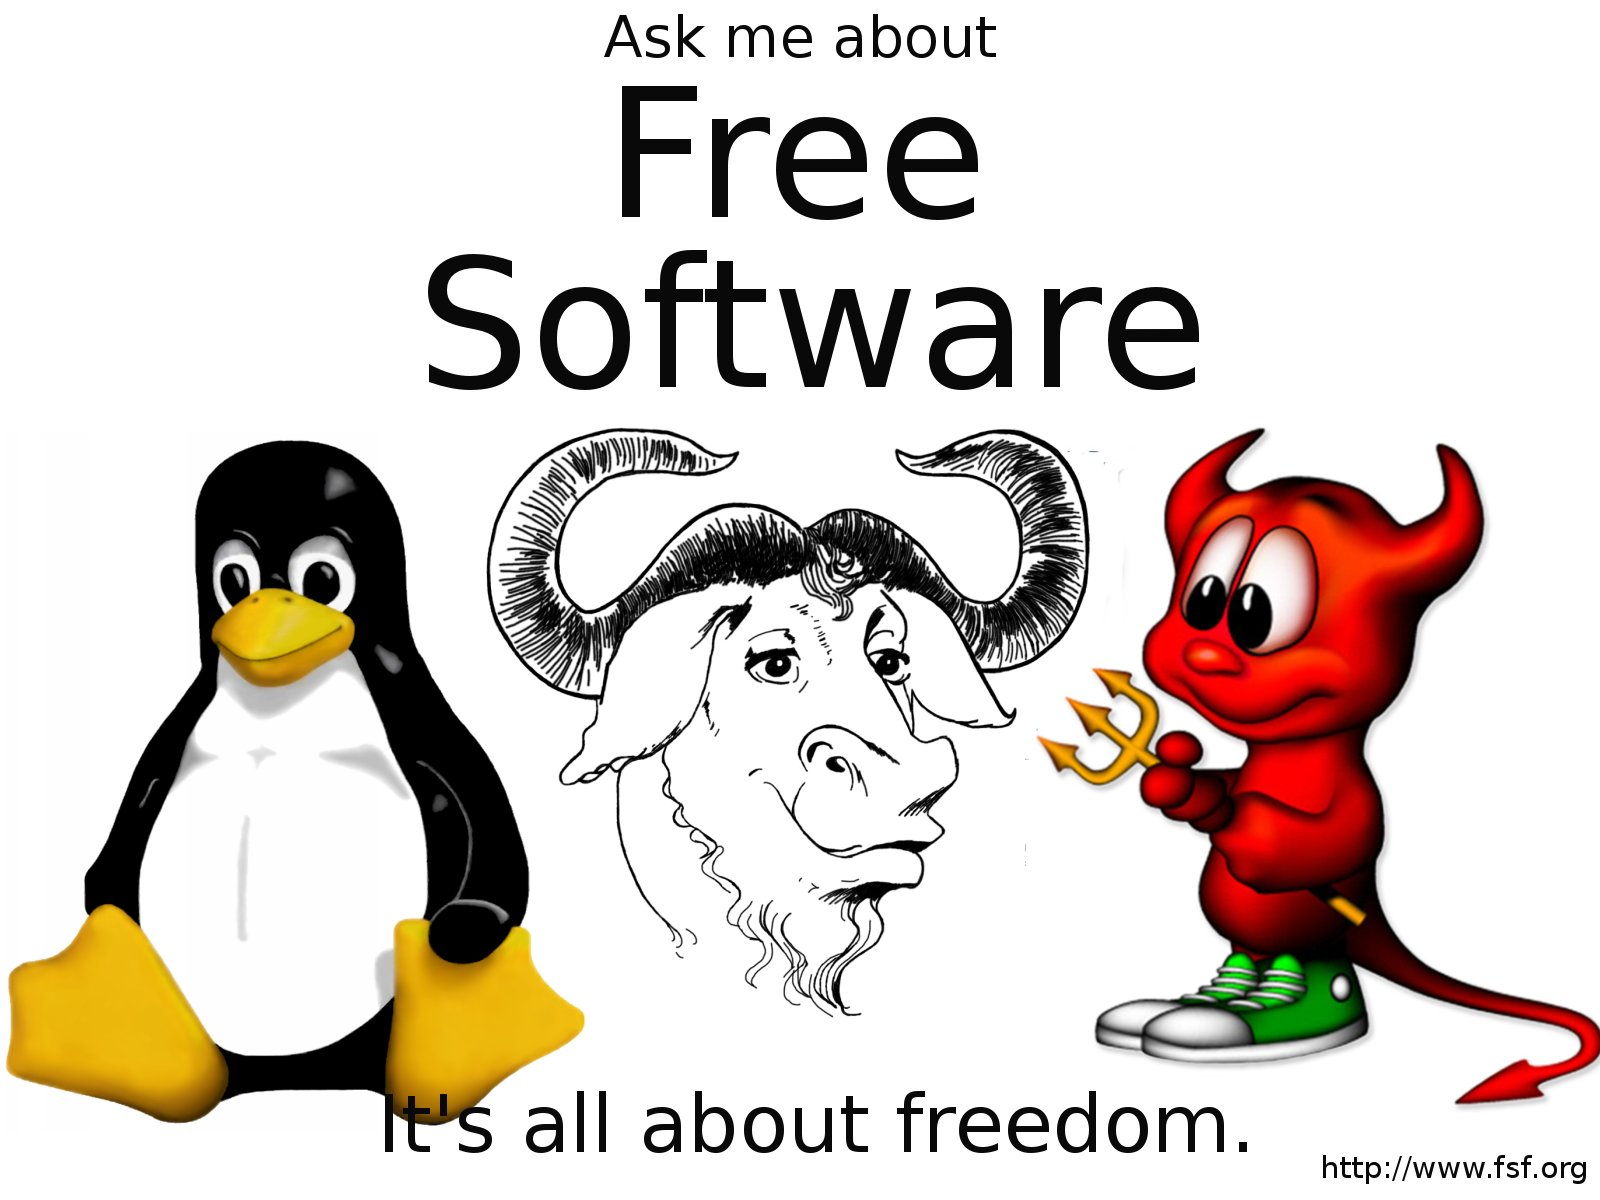
\includegraphics[width=.6\textwidth]{free-software.jpg}}
%=============================================================================
\date{}
\begin{document}
%========================= Title and outlines ================================
\begin{frame}{}
    \titlepage
\end{frame}

\newboolean{sectiontoc}
\setboolean{sectiontoc}{true} % default to true

\AtBeginSection[]
{
    \ifthenelse{\boolean{sectiontoc}}{
        \begin{frame}<beamer>
            \frametitle{Outline}
            \tableofcontents[currentsection,currentsubsection]
        \end{frame}
    }
}
\AtBeginSubsection[]
{
    \ifthenelse{\boolean{sectiontoc}}{
        \begin{frame}<beamer>
            \frametitle{Outline}
            \tableofcontents[currentsection,currentsubsection]
        \end{frame}
    }
}

%=============================================================================

%========================= Real presentation =================================
\begin{frame}{Outline}
    \tableofcontents
\end{frame}

\newsection{You said Free Software ?}


\begin{frame}{What is a software}
    % -
 %   Copyright (C) 2015  Beniamine, David <David@Beniamine.net>
 %   Author: Beniamine, David <David@Beniamine.net>
 %   
 %   This program is free software: you can redistribute it and/or modify
 %   it under the terms of the GNU General Public License as published by
 %   the Free Software Foundation, either version 3 of the License, or
 %   (at your option) any later version.
 %   
 %   This program is distributed in the hope that it will be useful,
 %   but WITHOUT ANY WARRANTY; without even the implied warranty of
 %   MERCHANTABILITY or FITNESS FOR A PARTICULAR PURPOSE.  See the
 %   GNU General Public License for more details.
 %   
 %   You should have received a copy of the GNU General Public License
 %   along with this program.  If not, see <http://www.gnu.org/licenses/>.
 %%

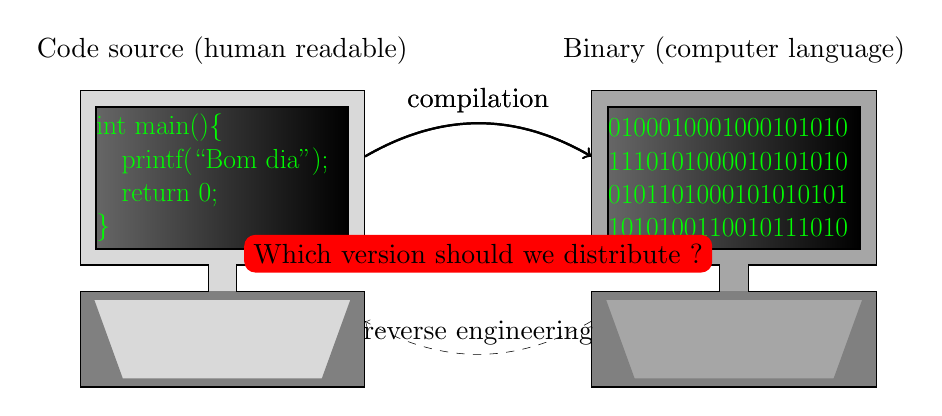
\begin{tikzpicture}

    \pic(code) at (.5,0) [draw, fill = gray!30,scale=.4,
    pic text ={
    int main()\{\\\quad printf(``Bom dia'');\\\quad return 0;\\\}}] {computer};
    \node[] at ($(code-c.north)+(0,.5)$) {Code source (human readable)};

    \uncover<2->{

        \pic (bin) [draw, fill = gray!70,scale=.4,
        pic text ={0100010001000101010
                   1110101000010101010
                   0101101000101010101
                   1010100110010111010}]
        at (0:7) {computer};
        \node[] at ($(bin-c.north)+(0,.5)$) {Binary (computer language)};

        \draw[->,thick] (code-c) to[bend left=30] node[above]{compilation} (bin-c);
    }

    \uncover<3->{
        \draw[->,thick] (code-c) to[bend left=30] node[above]{compilation} (bin-c);
    }

    \uncover<4->{
        \draw[->,very thin,dashed] (bin-c) to[bend left=30]  node[above]{reverse engineering} (code-c);
    }

    \uncover<5->{
        \node[fill=red, rounded corners,text centered] (q) at
        ($(code-c.south)+(3.25,1.7)$) {Which version should we distribute ?};
    }
\end{tikzpicture}

\end{frame}

\begin{frame}{What is Free Software}
    \begin{block}{Free Software Foundation definition~\cite{fsfdef}}
        \begin{itemize}[<+->]
            \item The freedom to run the program as you wish.
            \item The freedom to study how the program works.
            \item The freedom to redistribute.
            \item The freedom to distribute modified version.
        \end{itemize}
    \end{block}
    \uncover<5->{
    \begin{alertblock}{Richard M. Stallman}
        "Free software is a matter of liberty not price"
    \end{alertblock}
    }
\end{frame}

\begin{frame}{A bit of history}
    \begin{itemize}[<+->]
        \item 1983 R. M. Stallman announce GNU~\cite{RMSWeb}
        \item 1992 Linus Torvalds releases Linux kernel~\cite{Linux}
        \item 2013 M. Shuttleworth closes Ubuntu bug \#1~\cite{Bug1}
        \item Now fight continues, More:~\cite{fsfVideo}
    \end{itemize}
\end{frame}

\begin{frame}{Copy Left license}
    \begin{itemize}[<+->]
        \item GPL~\cite{GPL} Most used free Licence
        \item LGPL~\cite{LGPL} Same but does not force your code to be LGPL when including LGP sources
        \item WTFPL~\cite{WTFPL} Do what the fuck you want (not actual license)
        \item \dots
    \end{itemize}
\end{frame}


\begin{frame}{Free Software for a better world}
    \begin{columns}
        \begin{column}{.5\textwidth}
            \begin{itemize}[<+->]
                \item Security
                \item Data ?
                \item Avoid monopoles
                \item Collaborative work
                \item Fork for a better world
            \end{itemize}
        \end{column}
        \begin{column}{.5\textwidth}
            \uncover<2->
            {
                \begin{figure}
                    \centering
                    \includegraphics[width=\textwidth]{dog}
                    \caption{A dog~\cite{RMSDog}}
                \end{figure}
            }
        \end{column}
    \end{columns}
\end{frame}

\begin{frame}{Who use free software anyway ?}
    \begin{itemize}
        \item<1-> You
            \begin{itemize}
                \item Android
                \item Firefox
                \item Chrome(ium)
                \item VLC
            \end{itemize}
        \item<2-> Internet
        \item<3-> How many Linux are (hidden) in your house ?
    \end{itemize}
\end{frame}

\newsection{You said Linux ?}


\begin{frame}{You should said GNU/Linux}
    \resizebox{!}{.7\textheight}{
        \begin{centering}
            % -
 %   Copyright (C) 2015  Beniamine, David <David@Beniamine.net>
 %   Author: Beniamine, David <David@Beniamine.net>
 %   
 %   This program is free software: you can redistribute it and/or modify
 %   it under the terms of the GNU General Public License as published by
 %   the Free Software Foundation, either version 3 of the License, or
 %   (at your option) any later version.
 %   
 %   This program is distributed in the hope that it will be useful,
 %   but WITHOUT ANY WARRANTY; without even the implied warranty of
 %   MERCHANTABILITY or FITNESS FOR A PARTICULAR PURPOSE.  See the
 %   GNU General Public License for more details.
 %   
 %   You should have received a copy of the GNU General Public License
 %   along with this program.  If not, see <http://www.gnu.org/licenses/>.
 %%

\begin{tikzpicture}[
        scale=0.75,
        start chain=1 going below,
        start chain=2 going right,
        node distance=1mm,
        desc/.style={
            scale=0.75,
            on chain=2,
            rectangle,
            rounded corners,
            draw=black,
            very thick,
            text centered,
            text width=8cm,
            minimum height=12mm,
        },
        human/.style={
            fill=green
        },
        app/.style={
            fill=blue!60
        },
        preOS/.style={
            fill=blue!90
        },
        OS/.style={
            fill=orange!60
        },
        kern/.style={
            fill=orange
        },
        HW/.style={
            fill=red
        },
        level/.style={
            scale=0.75,
            on chain=1,
            minimum height=12mm,
            text width=5cm,
            text centered
        },
        every node/.style={font=\sffamily}
    ]

%layers
    \pgfdeclarelayer{background}
    \pgfdeclarelayer{foreground}
    \pgfsetlayers{background,main,foreground}

% Levels
    \begin{pgfonlayer}{foreground}

        \node [level] (user) {};

% Desktop env
        \uncover<6->{
            \node [level] (app) {Desktop Environment};
        }
        \uncover<2->{
            \node [level] (appEnv) {};
            \node [level] (appMgmt) {};
        }


        \uncover<3->{
            \node [level] (OS) {Operating System: GNU};
            \node [level] (OS1) {};
            \node [level] (OS2) {};
        }

        \uncover<4->{
            \node [level] (kern) {kernel: Linux};
            \node [level] (kern1) {};
        }

        \node [level] (HW) {Hardware};

% Description and groups
        \chainin (user);
        \node [desc,human] (UserDesc) {User};

% Desktop env
        \uncover<2->{
            \node [desc, continue chain=going below,app] (Applications) {Applications};
            \node [desc,app] (AppEnv) {Environment settings (windows decoration, interface)};
            \node [desc,preOS] (AppInst) {Applications installation and Management};
        }
    \end{pgfonlayer}

    \only<6->{
        \begin{pgfonlayer}{main}
            \node[draw,dotted,fit=(Applications) (appEnv),fill=blue!20]  (DEG) {};
        \end{pgfonlayer}
    }

    \begin{pgfonlayer}{foreground}
        \uncover<3->{
            \node [desc,OS] (OSHL) {Play sound, create window \dots};
            \node [desc,OS] (OSML) {Connect Network start application \dots};
            \node [desc,OS] (OSLL) {Open file, access Memory \dots};
        }
    \end{pgfonlayer}

    \only<5->{
        \begin{pgfonlayer}{main}
            \node[draw,dotted,fit=(OSHL) (kern1),fill=orange!20]  (OSG) {};
        \end{pgfonlayer}
    }

    \begin{pgfonlayer}{foreground}

        \uncover<4->{
            \node [desc,kern] (KernHL) {Process management \dots};
            \node [desc,kern] (KernLL) {Access RAM / Disk / Network \dots};
        }

        \node [desc,HW] (HW) {Computer};
    \end{pgfonlayer}

%Groups



% Distribution
    \only<7->{
        \begin{pgfonlayer}{main}
            \node[fit=(DEG) (OSG)]  (DISTI) {};
            \node[right=of DISTI.east]  (DISTT) {Distribution};
        \end{pgfonlayer}

        \begin{pgfonlayer}{background}
            \node[draw,dotted,fit=(DISTI) (DISTT), fill=green!20]  (DISTG) {};
        \end{pgfonlayer}
    }
\end{tikzpicture}

        \end{centering}
    }
\end{frame}

\begin{frame}{Distributions}
    \begin{centering}
        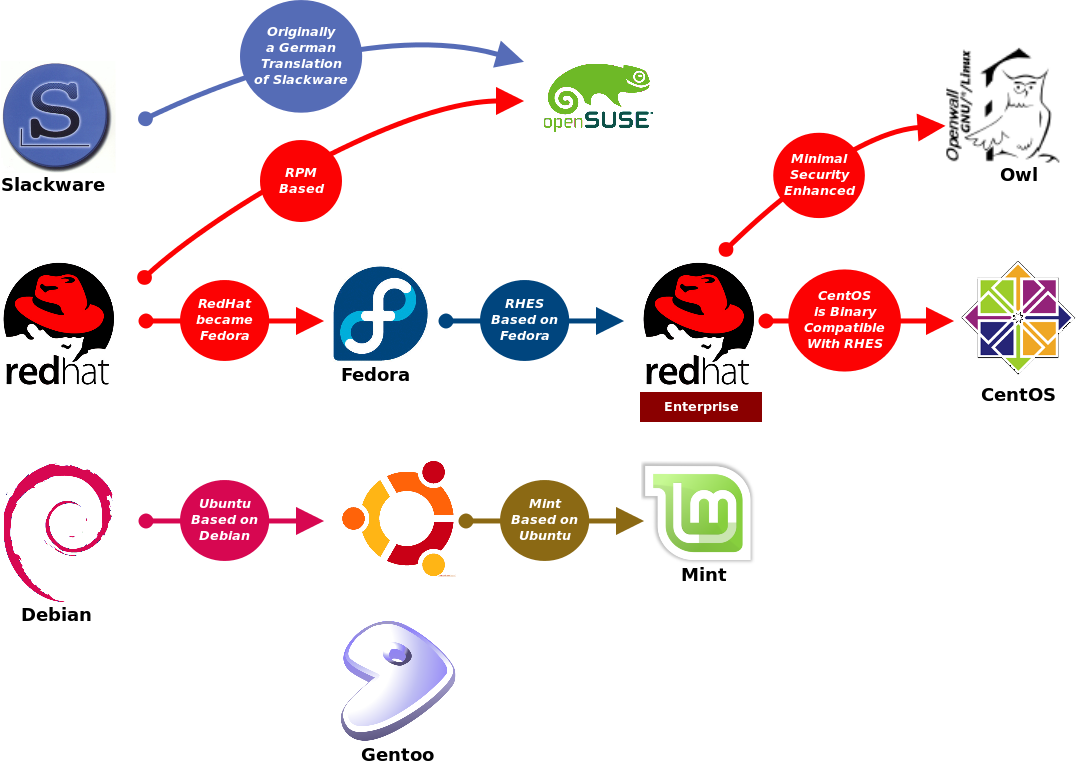
\includegraphics[width=.9\textwidth]{Major_distros}
    \end{centering}
\end{frame}

\begin{frame}{Policies}
    \begin{itemize}[<+->]
        \item Applications installation
        \item Release
        \item Support
    \end{itemize}
\end{frame}

\begin{frame}{Desktop environment}
    \begin{centering}
        
\includegraphics[width=.9\textwidth]{logo-Linux_environnements}
    \end{centering}
\end{frame}

\begin{frame}{Where to start ?}
    \begin{itemize}
        \item Ubuntu: easy way
        \item  Debian: control everything
        \item More~\cite{DistroWiki,DistroList}
    \end{itemize}
\end{frame}
\newsection{And now what ?}

\begin{frame}{Contribute}
    \begin{itemize}
        \item No need to be a dev
        \item Bug report
        \item Testing
        \item Translation
        \item Modification of documentation~\cite{ubdoc} / intervention in forums~\cite{ubforum}
        \item Talk to free softwares around you
    \end{itemize}
\end{frame}

\begin{frame}{Why is it only for computers ?}
    \begin{block}{It's not !}
        Creative commons~\cite{CC,CCWiki,DeviantArt}
    \end{block}
\end{frame}

\begin{frame}{Alternatives, Alternatives everywhere}
    \begin{itemize}
        \item Music player:
            \begin{itemize}
                \item Ryhtmbox
                \item Amarok
                \item Banshee
            \end{itemize}
        \item Pictures:
            \begin{itemize}
                \item Shotwell
                \item GIMP
            \end{itemize}
        \item Video
            \begin{itemize}
                \item VLC
                \item Pitivi
            \end{itemize}
        \item Social Networks
            \begin{itemize}
                \item Diaspora
            \end{itemize}
        \item Open Street maps
        \item Cloud
            \begin{itemize}
                \item Owncloud
            \end{itemize}
    \end{itemize}
\end{frame}

\newHsection{Conclusion}

\begin{frame}{Let's change the world !}
    \begin{block}{Let's install GNU/Linux}
        Or at least try it
    \end{block}
\end{frame}
\newcounter{finalframe}
\setcounter{finalframe}{\value{framenumber}}


%Last numbered frame go here
%=============================================================================

%=============================================================================
%Uncomment next lines for uncounted backup slides & biblio
\newHsection{Bibliography}
\setboolean{sectiontoc}{false}

\setcounter{framenumber}{\value{finalframe}}
\begin{frame}[allowframebreaks]
    \frametitle<presentation>{References}
    \begin{thebibliography}{10}
        %\setbeamertemplate{bibliography item}[online]
            \setbeamertemplate{bibliography item}[text]
            \bibitem{fsfdef}
            Free software definition
            \newblock \url{https://www.gnu.org/philosophy/free-sw.html}
            \bibitem{fsfVideo}
            Free Software Foundation explanation video
            \newblock \url{https://www.fsf.org/blogs/community/user-liberation-watch-and-share-our-new-video}
            \bibitem{RMSWeb}
            Richard M Stallman's website
            \newblock \url{https://www.stallman.org/}
            \bibitem{Linux}
            Linux original annouce
            \newblock
            \url{http://www.thelinuxdaily.com/2010/04/the-first-linux-announcement-from-linus-torvalds/}
            \bibitem{Bug1}
            Ubuntu Bug1
            \newblock \url{https://bugs.launchpad.net/ubuntu/+bug/1}
            \newblock  \url{https://bugs.launchpad.net/ubuntu/+bug/1/comments/1834}
            \bibitem{FSFWhatis}
            FSF: What is free software + Stallman speech
            \newblock \url{https://www.fsf.org/about/what-is-free-software}
            \bibitem{GPL}
            GPL License
            \newblock \url{https://www.gnu.org/licenses/gpl.html}
            \bibitem{LGPL}
            LGPL License
            \newblock \url{https://www.gnu.org/licenses/lgpl.html}
            \bibitem{WTFPL}
            What the fuck public license
            \newblock \url{http://www.wtfpl.net/}
            \bibitem{RMSDog}
            Dog image
            \newblock \url{https://www.stallman.org/images/dog.jpg}
            \bibitem{DistrosFull}
            Distribution timeline
            \newblock \url{http://futurist.se/gldt/}
            \bibitem{DistroWiki}
            Comparison of distributions
            \newblock \url{https://en.wikipedia.org/wiki/Comparison\_of\_Linux\_distributions}
            \bibitem{DistroList}
            List of distributions
            \newblock \url{https://en.wikipedia.org/wiki/List\_of\_Linux\_distributions}
            \bibitem{CC}
            Creative Commons
            \newblock \url{https://creativecommons.org/}
            \bibitem{DeviantArt}
            Deviant Art
            \newblock \url{http://www.deviantart.com/}
            \bibitem{CCWiki}
            Creative Commons License on wikipedia
            \newblock \url{http://en.wikipedia.org/wiki/Creative_Commons_license}
            \bibitem{ubforum}
            Ubuntu forums
            \newblock \url{http://ubuntuforums.org/}
            \newblock \url{http://ubuntuforum-br.org/}
            \bibitem{ubdoc}
            Ubuntu documentation
            \newblock \url{https://help.ubuntu.com/community/}
            \newblock \url{https://help.ubuntu.com/}
            \newblock \url{http://wiki.ubuntu-br.org/}
    \end{thebibliography}
\end{frame}

%%
%\bibliographystyle{apalike}
%\bibliography{presentation}

%========================= Backup slides =====================================
%\newsection*{Hidden slides}
%put this line before each frame
%\setcounter{framenumber}{\value{finalframe}}

%=============================================================================
\end{document}
